\documentclass[11pt,a4paper]{article}

\usepackage[margin=2.4cm]{geometry}
\usepackage[T1]{fontenc}
\usepackage{amsmath,amssymb}
\usepackage{graphicx}
\usepackage{booktabs}
\usepackage{siunitx}
\usepackage{caption}
\usepackage{subcaption}
\usepackage{xcolor}
\usepackage[colorlinks=true,linkcolor=blue!50!black,citecolor=blue!50!black,urlcolor=blue!50!black]{hyperref}
\usepackage{listings}
\usepackage{enumitem}
\setlist{itemsep=1pt,topsep=2pt}

\lstset{
  basicstyle=\ttfamily\footnotesize,
  breaklines=true,
  frame=single,
  language=Python,
  showstringspaces=false,
}

\title{Operations Optimisation Assignment\\
\large Reproducing the MILP for the Drone-Assisted Pickup and Delivery Problem\\
{\small Mulumba \& Diabat, \emph{Transp. Res. E} 181 (2024) 103377}}
\author{Rohit Roy Chowdhury, Swayam Kuckreja (5726549), Kai Murtagh (5685095)\\TU Delft Aerospace Engineering}
\date{July 2026}

\newcommand{\R}{\mathbb{R}}
\newcommand{\Nplus}{N^{+}}
\newcommand{\NO}{N^{0}}
\newcommand{\Cprime}{C'}
\newcommand{\E}{\mathcal{E}}
\newcommand{\dapdp}{\textsc{DAPDP}}
\newcommand{\pdp}{\textsc{PDP}}

\begin{document}
\maketitle

\section{Introduction}

This report reproduces the mixed-integer linear program of Mulumba and
Diabat~\cite{mulumba2024} for the Drone-Assisted Pickup and Delivery Problem
(\dapdp). A truck performs a sequence of paired pickup and delivery requests
while a single on-board drone may peel off, deliver a light parcel, and
rendezvous with the truck downstream. The goal is to minimise total fuel cost
subject to truck capacity, drone payload and endurance, and a maximum route
duration.

The contributions of this work are:
\begin{enumerate}
\item A clean Python/Gurobi implementation of all $37$ constraints of the
paper (Section~3.2 of the original) plus two of the three valid-inequality
families of Section~3.3: the cost-bound epigraph (Prop.~1) and the knapsack
cuts~(43)--(44). The symmetry-breaking cut~(41)--(42) is omitted because it
is nonlinear (a product $u^{v}_{i}\,x^{v}_{0i}$) and so not directly
expressible in the MILP.
\item A truck-only baseline obtained by restricting the same model with
$\Cprime{=}\emptyset$, used to compute the saving $\mathit{SPDP} = 1 -
z_{\dapdp} / z_{\pdp}$.
\item A verification suite of seven independently-audited test scenarios
covering each major class of constraint.
\item A sensitivity analysis on drone endurance, drone speed and the drone
cost factor $\alpha$.
\item A small-scale validation on the paper's instance sizes
$n \in \{6, 8, 10\}$, which reproduces the qualitative finding that the drone
yields positive cost savings. The mean SPDP across these small cells is
$\approx 14\%$; the paper's headline $\approx 25\%$ is an average over its
\emph{large}-scale set (up to $n{=}150$), and our smaller, grid-dependent
savings are consistent with the paper's own small-instance rows
(Table~A.6).
\end{enumerate}

The paper contains a small number of typographic ambiguities
(constraint~(28), the demand sign convention in \S5.2, and the launch-side
treatment in constraints~(10) and~(26)) which we resolve and document
explicitly in \S\ref{sec:interpretations}.

\paragraph{Reproducibility.}
A single shell script \texttt{run\_all.sh} regenerates every CSV, PDF
figure and the report itself from scratch. All numerical values reported
below come directly from the most recent run of that script.

\section{Problem statement}

Let $\Nplus = \{1,\dots,2n+1\}$, $\NO = \{0,\dots,2n\}$, $C =
\{1,\dots,2n\}$ be the customer node set, partitioned into pickups
$\Phi^{+} = \{1,\dots,n\}$ and deliveries $\Phi^{-} = \{n{+}1,\dots,2n\}$;
delivery node $n{+}i$ is paired with pickup $i$. Node $0$ is the start
depot, node $2n{+}1$ a virtual end depot at the same location. The
drone-eligible subset $\Cprime \subseteq \Phi^{-}$ contains those
deliveries whose demand $\le Q'$, the drone payload limit. Truck travel
time is $\tau_{ij} = d_{ij}/s$, drone travel time $\tau'_{ij} = d_{ij}/s'$
with $d_{ij}$ the Euclidean distance.

\paragraph{Demand sign convention.}
We use $q_i > 0$ at pickups and $q_i < 0$ at deliveries. This is the
\emph{opposite} of the textual statement in the paper's \S5.2 but is the
only convention consistent with the literal reading of the weight
balance~(28), where positive contributions of $q_j$ must increase the
truck load on arrival.

\paragraph{Decision variables.}
\begin{itemize}
\item $x^{v}_{ij}\in\{0,1\}$: truck $v$ traverses arc $(i,j)$.
\item $y^{v}_{ijk}\in\{0,1\}$: a drone-sortie launch $i$, drone delivery
$j$, rendezvous $k$ for truck $v$.
\item $p^{v}_{ij}\in\{0,1\}$: $i$ precedes $j$ in truck $v$'s route.
\item $t^{v}_{i},\;t'^{\,v}_{i}\ge 0$: truck and drone arrival times at $i$.
\item $u^{v}_{i}\in\{1,\dots,|N|\}$: position of $i$ in truck $v$'s
sequence.
\item $w^{v}_{i}\ge 0$: truck weight after visiting $i$.
\item $\eta\ge 0$: epigraph variable; objective $\min \eta$ with $\eta \ge
\sum_{v,i,j} c_{ij}x^{v}_{ij} + \sum_{v,(i,j,k)\in P}
(c'_{ij}{+}c'_{jk}) y^{v}_{ijk}$.
\end{itemize}

\paragraph{Mathematical model.}
The implemented MILP is given below in the paper's equation numbering, with
the deviations of \S\ref{sec:interpretations} already folded in (the
$-M$ sign in~(28), the epigraph objective~(38)--(39), the depot-launch ban
in~(26), and the elision of~(10) and~(35)). Two big-$M$ constants are used:
$M_{\mathrm{pos}}=2n{+}2$ in the position constraints and
$M_t=T_{\max}+10$\,h in the time constraints. The drone sortie set is
$\mathcal P=\{(i,j,k):i\ne 0,\;j\in\Cprime,\;k\in\Nplus,\;i,j,k\text{
distinct}\}$, pre-filtered for endurance.
{\footnotesize
\allowdisplaybreaks
\begin{align}
& \min~ \eta \tag{38}\\
& \eta \ge \sum_{v\in\mathcal V}\Big(\sum_{(i,j)\in\mathcal A} c_{ij}x^{v}_{ij}
   +\sum_{i\in\NO}\sum_{j\in C}\sum_{k\in\Nplus}(c'_{ij}+c'_{jk})\,y^{v}_{ijk}\Big) \tag{39}\\
& \sum_{v}\Big(\sum_{i\in\NO:i\ne j}x^{v}_{ij}
   +\sum_{i\in\NO:i\ne j}\sum_{k\in\Nplus}y^{v}_{ijk}\Big)=1,
   \quad \forall j\in C \tag{2}\\
& \sum_{j\in\Nplus}x^{v}_{0j}\le 1,\quad
  \sum_{i\in\NO}x^{v}_{i,2n+1}\le 1,
   \qquad \forall v \tag{3,4}\\
& 1+u^{v}_{i}-u^{v}_{j}\le(1-x^{v}_{ij})\,M_{\mathrm{pos}},
   \quad \forall i\in C,\,j\in\Nplus\!\setminus\!\{i\},\,v \tag{5}\\
& \sum_{i\in\NO:i\ne j}x^{v}_{ij}=\sum_{k\in\Nplus:k\ne j}x^{v}_{jk},
   \quad \forall j\in C,\,v \tag{6}\\
& \sum_{j\in C:j\ne i}\sum_{k\in\Nplus}y^{v}_{ijk}\le 1,\;\;\forall i\in\NO;\quad
  \sum_{i\in\NO:i\ne k}\sum_{j\in C}y^{v}_{ijk}\le 1,\;\;\forall k\in\Nplus \tag{7,8}\\
& 2y^{v}_{ijk}\le \textstyle\sum_{h\in\NO:h\ne i}x^{v}_{hi}
   +\sum_{l\in\NO:l\ne k}x^{v}_{lk},
   \quad \forall (i,j,k)\in\mathcal P,\,v
   \;\;\text{(launch term}\equiv 1\text{ if }i{=}0) \tag{9}\\
& u^{v}_{k}-u^{v}_{i}\ge 1-M_{\mathrm{pos}}\big(1-\textstyle\sum_{j}y^{v}_{ijk}\big),
   \quad \forall i\in C,\,k\in\Nplus\!\setminus\!\{i\},\,v \tag{11}\\
& t'^{\,v}_{i}\ge t^{v}_{i}-M_t\big(1-\textstyle\sum_{j,k}y^{v}_{ijk}\big),\quad
  t'^{\,v}_{i}\le t^{v}_{i}+M_t\big(1-\textstyle\sum_{j,k}y^{v}_{ijk}\big),
   \;\; \forall i\in C,\,v \tag{12,13}\\
& t'^{\,v}_{k}\ge t^{v}_{k}-M_t\big(1-\textstyle\sum_{i,j}y^{v}_{ijk}\big),\quad
  t'^{\,v}_{k}\le t^{v}_{k}+M_t\big(1-\textstyle\sum_{i,j}y^{v}_{ijk}\big),
   \;\; \forall k\in C,\,v \tag{14,15}\\
& t^{v}_{k}\ge t^{v}_{h}+\tau_{hk}+d_{h}
   +s_{L}\!\textstyle\sum_{l,m}y^{v}_{klm}
   +s_{R}\!\textstyle\sum_{i,j}y^{v}_{ijk}-M_t(1-x^{v}_{hk}),
   \;\; \forall h\in\NO,\,k\in\Nplus\!\setminus\!\{h\},\,v \tag{16}\\
& t'^{\,v}_{j}\ge t'^{\,v}_{i}+\tau'_{ij}-M_t\big(1-\textstyle\sum_{k}y^{v}_{ijk}\big),
   \quad \forall j\in\Cprime,\,i\in\NO\!\setminus\!\{j\},\,v \tag{17}\\
& t'^{\,v}_{k}\ge t'^{\,v}_{j}+\tau'_{jk}+d'_{j}+s_{R}
   -M_t\big(1-\textstyle\sum_{i}y^{v}_{ijk}\big),
   \quad \forall j\in\Cprime,\,k\in\Nplus\!\setminus\!\{j\},\,v \tag{18}\\
& t'^{\,v}_{k}-(t'^{\,v}_{j}-\tau'_{ij})\le e+M_t(1-y^{v}_{ijk}),
   \quad \forall (i,j,k)\in\mathcal P,\,v \tag{19}\\
& u^{v}_{i}-u^{v}_{j}\ge 1-M_{\mathrm{pos}}\,p^{v}_{ij},\quad
  u^{v}_{i}-u^{v}_{j}\le -1+(1-p^{v}_{ij})\,M_{\mathrm{pos}},
   \;\; \forall i,j\in C:i\ne j,\,v \tag{20,21}\\
& p^{v}_{ij}+p^{v}_{ji}=1,\quad \forall i,j\in C:i<j,\,v \tag{22}\\
& t'^{\,v}_{l}\ge t'^{\,v}_{k}-M_t\big(3-\textstyle\sum_{j}y^{v}_{ijk}
   -\sum_{m,n}y^{v}_{lmn}-p^{v}_{il}\big),
   \;\; \forall i\in\NO,\,k\in\Nplus\!\setminus\!\{i\},\,l\in C\!\setminus\!\{i,k\},\,v \tag{23}\\
& x^{v}_{0,2n+1}=0,\quad \forall v \tag{24}\\
& \sum_{j\in\Nplus:j\ne i}x^{v}_{ij}=\sum_{j\in\Nplus:j\ne n+i}x^{v}_{n+i,j}
   +\sum_{l\in\NO}\sum_{k\in\Nplus}y^{v}_{l,n+i,k},
   \quad \forall i\in\Phi^{+},\,v \tag{25}\\
& u^{v}_{i}-u^{v}_{j-n}\ge 1-M_{\mathrm{pos}}(1-y^{v}_{ijk}),
   \;\; \forall (i,j,k)\in\mathcal P,\,j\in\Phi^{-};\qquad y^{v}_{0jk}=0 \tag{26}\\
& t^{v}_{n+i}\ge t^{v}_{i}+\tau_{i,n+i}+d_{i},
   \quad \forall i\in\Phi^{+},\,v \tag{27}\\
& w^{v}_{j}\ge w^{v}_{i}+q_{j}
   +\!\!\sum_{(j,m,k)\in\mathcal P}\!\! q_{m}\,y^{v}_{jmk}-Q(1-x^{v}_{ij}),
   \;\; \forall i\in\NO,\,j\in C:i\ne j,\,v \tag{28}\\
& t^{v}_{0}=t'^{\,v}_{0}=0;\quad
  t^{v}_{2n+1}\le T_{\max},\;\; t'^{\,v}_{2n+1}\le T_{\max},
   \quad \forall v \tag{31--34}\\
& 1\le u^{v}_{i}\le 2n{+}2,\quad 0\le w^{v}_{i}\le Q \tag{36,37}\\
& x^{v}_{ij}+\textstyle\sum_{k\in\Nplus}y^{v}_{ijk}\le 1,
   \quad \forall i\in\NO,\,j\in\Cprime:i\ne j,\,v \tag{43}\\
& x^{v}_{ij}+x^{v}_{jk}+x^{v}_{ik}+y^{v}_{ijk}\le 2,
   \quad \forall (i,j,k)\in\mathcal P,\,v \tag{44}
\end{align}}%
Variables are binary ($x,y,p$) or non-negative continuous ($t,t',w,\eta$),
with $u$ integer. Table~\ref{tab:constraints} summarises the role of each
group; the non-obvious implementation choices are detailed next.

\begin{table}[t]
\centering
\caption{Constraint groups of the \dapdp{} MILP and their implementation.}
\label{tab:constraints}
\small
\begin{tabular}{@{}lll@{}}
\toprule
Eqs.        & Purpose                                          & Implementation note \\
\midrule
(2)         & Each customer served exactly once                & --- \\
(3)--(4)    & Depot start/end at most once per truck           & --- \\
(5)         & Sub-tour elimination (MTZ on $u$)                & big-$M_{\text{pos}} = 2n+2$ \\
(6)         & Truck flow conservation                          & --- \\
(7)--(8)    & At most one launch/return per node               & --- \\
(9)--(10)   & Launch and rendezvous on truck route             & (10) subsumed by (9), see \S\ref{sec:interpretations} \\
(11)        & Launch precedes rendezvous in $u$                & --- \\
(12)--(15)  & Time synchronisation of truck and drone          & big-$M_t = T_{\max}+10$\,h \\
(16)        & Truck-arrival recursion (with launch/recovery)   & --- \\
(17)--(18)  & Drone-arrival recursion                          & --- \\
(19)        & Drone endurance $\le e$                          & also pre-filtered into $P$ \\
(20)--(22)  & Consistency of $u$ and $p$                       & --- \\
(23)        & No second sortie before return of first          & --- \\
(24)        & Forbid empty depot-to-depot trip                 & --- \\
(25)        & Same vehicle for paired (i, $i+n$)               & --- \\
(26)        & Pickup before launch when drone delivers $j$     & extended to $i{=}0$, see \S\ref{sec:interpretations} \\
(27)        & Pickup precedes delivery on truck                & --- \\
(28)        & Truck weight evolution                           & sign correction, see \S\ref{sec:interpretations} \\
(31)--(34)  & Time bounds, $T_{\max}$                          & --- \\
(35)        & $p^{v}_{0j}=1$                                   & omitted; see \S\ref{sec:interpretations} \\
(36)--(37)  & Bounds on $u, w$                                 & encoded in variable bounds \\
(43)--(44)  & Knapsack valid inequalities (Section 3.3)        & on; symmetry cut (41) omitted (nonlinear) \\
\bottomrule
\end{tabular}
\end{table}

\section{Interpretation decisions where the paper is ambiguous}
\label{sec:interpretations}

The paper has a few places where the printed model is either
mathematically inconsistent or requires assumptions that are not stated.
Implementing it verbatim would yield an infeasible or trivially-relaxed
program, so we deviate as follows.

\paragraph{(28) Truck weight balance --- big-$M$ sign.}
The paper writes
\[
w^{v}_{j} \ge w^{v}_{i} + q_{j} + \sum_{(i,j,k)\in P} q_{m}\,y^{v}_{j m k}
\;{\color{red}+}\;Q\,(1 - x^{v}_{ij}),
\]
which has the wrong sign of the big-$M$. With $+M$, every arc with
$x^{v}_{ij}=0$ would force $w^{v}_{j} \le w^{v}_{i} + q_{j} + \dots - Q$
(re-arranging), which is structurally infeasible whenever $Q$ is large.
The standard relaxation is $-M(1-x^{v}_{ij})$, which deactivates the
inequality whenever the arc is unused. We implement this minus sign.

\paragraph{Demand-sign convention.}
The paper's \S5.2 says ``demand $q_i$ is randomly drawn from $U(0, 2.27)$
with probability 0.86 \dots and the pickup demand is $-q_{n+i}$.'' Taking
this literally gives $q^{+} < 0$ at pickups and $q^{-} > 0$ at deliveries,
which contradicts (28) (truck load should \emph{rise} on a pickup). We
adopt the sign convention required by (28) and described in our
\texttt{instance\_generator.py}: $q_i > 0$ at pickup, $q_i < 0$ at delivery.

\paragraph{(26) Pickup-before-launch: depot launches.}
Constraint~(26) reads $u^{v}_{i} - u^{v}_{j-n} \ge 1 - M(1{-}y^{v}_{ijk})$
for $j\in\Phi^{-}$, $i\in C$. Two issues arise. First, $i$ runs over $C$
only, so $i=0$ is implicitly excluded; nothing in the paper prevents
launching a delivery sortie directly from the depot, which would let the
drone deliver before the truck has performed the corresponding pickup.
Second, when $i \in C$ but the corresponding pickup $j-n$ has not been
visited yet, $u^{v}_{j-n}$ is undefined relative to $u^{v}_{i}$. We
strengthen (26) by setting $y^{v}_{0jk}=0$ for every $j\in\Phi^{-}$,
$k\in\Nplus$. With one truck this rules out the only physically
non-implementable depot-launch case, and matches the paper's heuristic
(Algorithm~4) which only considers post-pickup launches.

\paragraph{(10) is subsumed by (9).}
Constraint~(10), $\sum_{i,j} y^{v}_{0jk} \le \sum_{l\ne k} x^{v}_{lk}$,
demands the rendezvous $k$ be on the truck route when the launch is from
the depot. Constraint~(9) already requires that, with the convention
$\mathbb{1}\{i\in\text{route}\}=1$ for $i=0$. We therefore implement only
(9) and document this elision.

\paragraph{(35) is omitted.}
Constraint~(35), $p^{v}_{0,j}=1$ for all $j\in C$, requires precedence
variables on the depot. We omit it because all our other depot-linked
constraints (the MTZ inequality, time/position bounds and (3)--(4)) place
the depot first implicitly. Including (35) would require tracking
$p^{v}_{0j}$ throughout, which inflates the variable count by $|C|$
without changing the feasible set.

\paragraph{$P$ pre-filtering.}
We pre-filter the universe of sorties $P = \{(i,j,k): i\ne 0,\;j \in
\Cprime,\;k\in\Nplus,\;i,j,k\text{ distinct}\}$ to those satisfying
$s_L + (d_{ij}+d_{jk})/s' + d^{\,\text{drone}}_{j} + s_R \le e$. Sorties
that fail this geometric check are forbidden by~(19) anyway, but
filtering them out shrinks the model by roughly an order of magnitude.

\section{Implementation}

The Python package is organised as
\begin{itemize}
\item \texttt{instance\_generator.py}: random-instance factory matching
\S5.2 of the paper (Table~1 defaults), plus a manual constructor used by
the verification suite.
\item \texttt{dapdp\_model.py}: the MILP, exposing
\texttt{solve\_dapdp(inst, time\_limit, ...)} that returns a
\texttt{Solution} dataclass.
\item \texttt{baseline.py}: solves the same MILP with $\Cprime=\emptyset$
to obtain $z_{\pdp}$ for SPDP computation.
\item \texttt{verification.py}: seven scenarios, each producing a
matplotlib figure plus an independently audited feasibility report.
\item \texttt{sensitivity.py}: parameter sweeps with CSV and PDF output.
\item \texttt{validation.py}: small-scale comparison with
$\overline{\mathit{SPDP}}$ values reported in the paper.
\end{itemize}

The solver is Gurobi 13.0.2 with a TU Delft academic licence. Instance
sizes up to $n{=}10$ on a $30{\times}30$\,mile grid solve to optimality in
seconds-to-minutes, comparable to the runtimes reported in the paper for
the corresponding sizes.

\section{Verification}
\label{sec:verification}

Following the assignment guidelines, we devise instances whose feasible
solutions are restricted in a well-understood way and verify the solver
respects those restrictions. Each scenario is paired with an independent
auditor (\texttt{audit()} in \texttt{verification.py}) that re-derives
feasibility from the returned $x$ and $y$ values without using any
internal solver state.

\subsection{Scenarios}

\begin{description}[style=nextline,leftmargin=2em]
\item[V1, basic feasibility ($n{=}3$).] A randomly generated instance.
The auditor checks every constraint listed in
Table~\ref{tab:constraints}. Result: \emph{passed}, $z^{\star}=\$0.91$,
runtime $0.3$\,s. Figure~\ref{fig:V1}.

\item[V2, pickup-precedence (handcrafted).] All demands set to $5$\,kg
($>Q'$), so $\Cprime=\emptyset$ and the truck must serve every pair. The
auditor confirms each delivery follows its pickup in the truck sequence:
route $0\to1\to2\to3\to6\to5\to4\to7$. Figure~\ref{fig:V2}.

\item[V3, endurance.] The same instance solved with $e=60$\,min and
$e=5$\,min. With generous endurance the solver uses $2$ drone sorties
($z^{\star}=\$4.65$); with the $5$\,min limit no sortie is feasible
($z^{\star}=\$5.34$, $0$ sorties). Figure~\ref{fig:V3}. Both audits pass.

\item[V4, drone payload.] Three deliveries with demands $\{1, 50, 1\}$
kg. Only deliveries $4$ and $6$ are in $\Cprime$. The drone serves
exclusively delivery $6$; delivery $5$ (heavy) is on the truck route.
Figure~\ref{fig:V4}.

\item[V5, no sub-tours ($n{=}6$).] Verifies the truck's arc set forms a
single connected path $0\to\dots\to 2n{+}1$ with no detached cycles.
Figure~\ref{fig:V5}.

\item[V6, $z_{\dapdp}\le z_{\pdp}$.] Same instance ($n{=}8$, grid $10$,
seed $3$) solved twice. The DAPDP optimum strictly improves on the PDP
baseline; the achieved saving is reported in
Table~\ref{tab:verification}. Figure~\ref{fig:V6}.

\item[V7, no depot-launch deliveries.] After our extension of (26),
$y^{v}_{0jk}=0$ for $j\in\Phi^{-}$. The auditor confirms no drone sortie
in the optimum has $i=0$.
\end{description}

\begin{figure}[t]
\centering
\begin{subfigure}{0.46\textwidth}
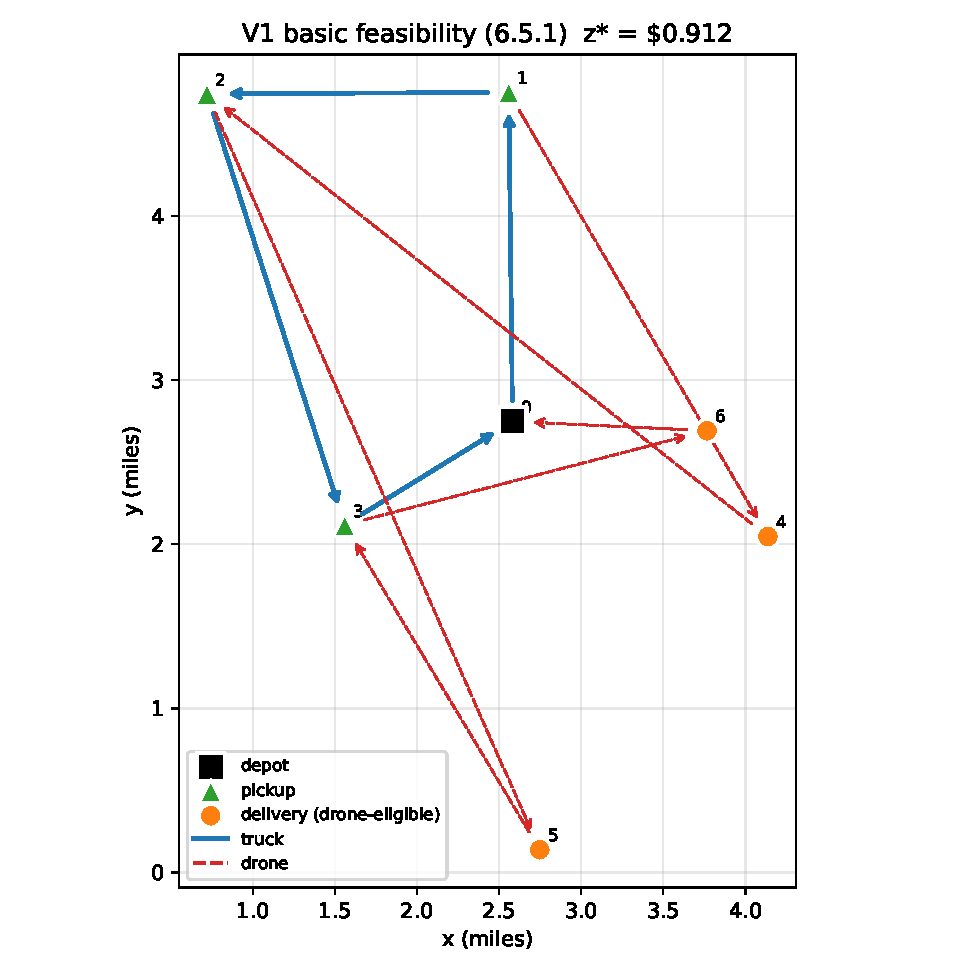
\includegraphics[width=\linewidth]{figures/V1_basic.pdf}
\caption{V1 basic feasibility, $n{=}3$.}
\label{fig:V1}
\end{subfigure}\hfill
\begin{subfigure}{0.46\textwidth}

\includegraphics[width=\linewidth]{figures/V2_pickup_precedence.pdf}
\caption{V2 pickup-before-delivery (drone disabled).}
\label{fig:V2}
\end{subfigure}
\caption{Verification scenarios V1 and V2.}
\end{figure}

\begin{figure}[t]
\centering
\begin{subfigure}{0.46\textwidth}

\includegraphics[width=\linewidth]{figures/V3_endurance_60min.pdf}
\caption{$e=60$\,min: $2$ sorties, $z^{\star}=\$4.65$.}
\end{subfigure}\hfill
\begin{subfigure}{0.46\textwidth}

\includegraphics[width=\linewidth]{figures/V3_endurance_05min.pdf}
\caption{$e=5$\,min: $0$ sorties, $z^{\star}=\$5.34$.}
\end{subfigure}
\caption{V3 endurance test on the same instance.}
\label{fig:V3}
\end{figure}

\begin{figure}[t]
\centering
\begin{subfigure}{0.46\textwidth}
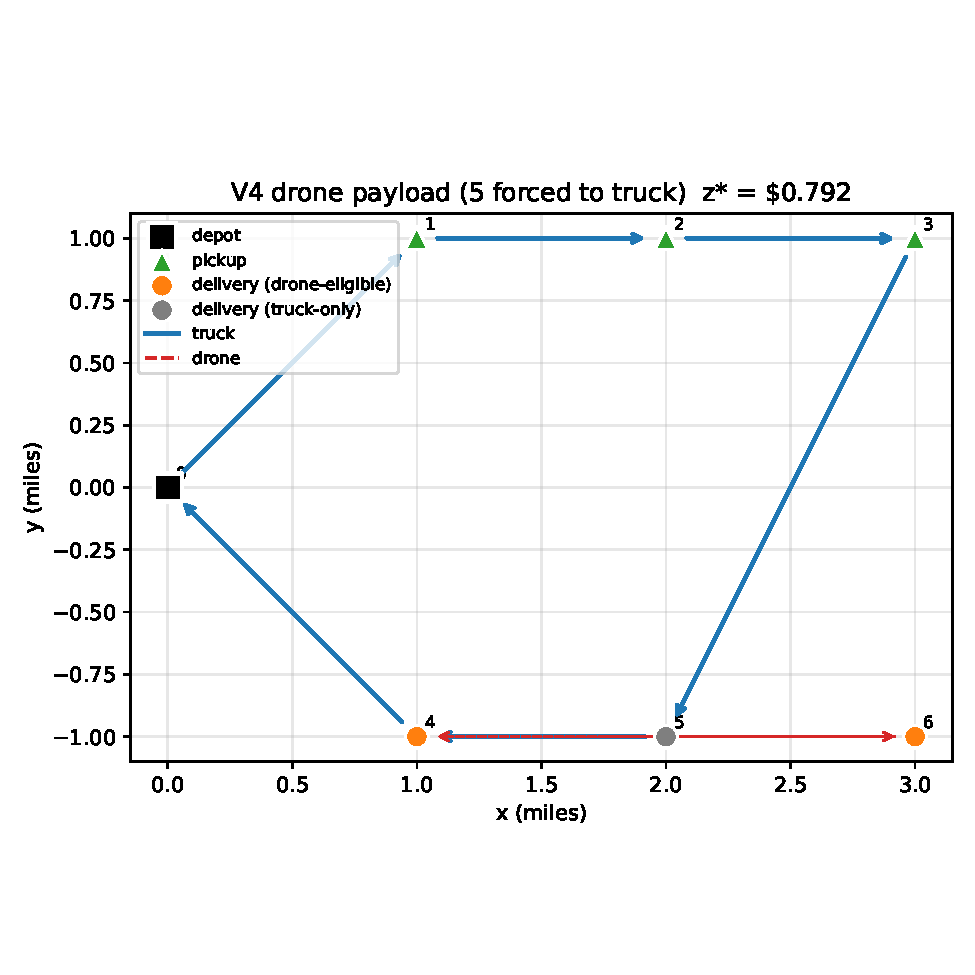
\includegraphics[width=\linewidth]{figures/V4_drone_payload.pdf}
\caption{V4: heavy delivery (5) excluded from $\Cprime$.}
\label{fig:V4}
\end{subfigure}\hfill
\begin{subfigure}{0.46\textwidth}

\includegraphics[width=\linewidth]{figures/V5_no_subtours.pdf}
\caption{V5 sub-tour elimination ($n{=}6$).}
\label{fig:V5}
\end{subfigure}
\caption{Verification scenarios V4 and V5.}
\end{figure}

\begin{figure}[t]
\centering
\begin{subfigure}{0.46\textwidth}

\includegraphics[width=\linewidth]{figures/V6_pdp.pdf}
\caption{Truck-only \pdp{} baseline.}
\end{subfigure}\hfill
\begin{subfigure}{0.46\textwidth}

\includegraphics[width=\linewidth]{figures/V6_dapdp.pdf}
\caption{\dapdp{} optimum (saving over PDP shown in Table~\ref{tab:verification}).}
\end{subfigure}
\caption{V6: same instance, both formulations.}
\label{fig:V6}
\end{figure}

\subsection{Audit summary}
\begin{table}[h]
\centering
\caption{Verification suite results, produced by \texttt{verification.py}
with the academic licence. For V6 the $z^\star$ column reports the DAPDP
optimum; the truck-only baseline is $z_{\pdp}=\$4.316$, giving a saving
$S_{\pdp}=1-3.011/4.316\approx 30\%$.}
\label{tab:verification}
\small
\begin{tabular}{@{}llrrl@{}}
\toprule
ID & description                       & $z^\star$ (\$) & runtime (s) & verdict \\
\midrule
V1 & basic, $n{=}3$                    & $0.912$ & $0.3$ & passed \\
V2 & pickup-precedence (truck only)    & $0.914$ & $0.5$ & passed \\
V3a & endurance 60 min                 & $4.652$ & $0.6$ & passed (2 sorties) \\
V3b & endurance 5 min                  & $5.341$ & $0.6$ & passed (0 sorties) \\
V4 & drone payload                     & $0.792$ & $0.4$ & passed (drone serves only $\{6\}$) \\
V5 & no sub-tours, $n{=}6$             & $4.715$ & $8.0$ & passed (single path) \\
V6 & DAPDP $\le$ PDP, $n{=}8$          & $3.011$ & $218.0$ & passed ($S_{\pdp}\approx 30\%$) \\
V7 & no depot-launch deliveries        & $0.664$ & $0.4$ & passed (no $y_{0jk}{=}1$) \\
\bottomrule
\end{tabular}
\end{table}

\section{Sensitivity analysis}
\label{sec:sensitivity}

We sweep three parameters that the paper highlights as most influential. The
ensemble is $12$ instances ($n\in\{6,8\}$, grid sizes $\{10,20\}$\,miles,
seeds $\{1,2,3\}$); $z_{\pdp}$ is computed once per instance and cached, so
each sweep value is one DAPDP solve per instance.

\subsection{Endurance}

Figure~\ref{fig:sens_endurance} shows mean SPDP rising monotonically with
endurance and saturating around $30$\,min, the paper's nominal value.
This matches the paper's Table~3 / Figure~9: when the drone can fly long
enough to serve more eligible deliveries, savings approach a ceiling
imposed by the drone's payload and route geometry.

\begin{figure}[h]
\centering
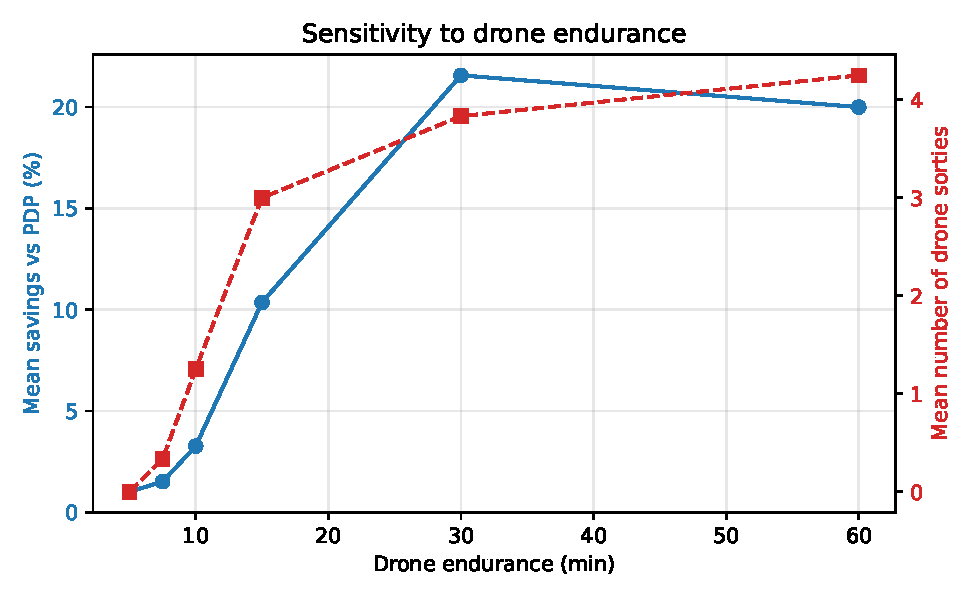
\includegraphics[width=0.6\textwidth]{figures/endurance.pdf}
\caption{Sensitivity of SPDP and number of sorties to drone endurance.}
\label{fig:sens_endurance}
\end{figure}

\subsection{Drone speed}

Figure~\ref{fig:sens_speed}: faster drones save more, but the relationship
flattens above $50$\,mph because most of the savings come from the
\emph{routing detour avoided} on the truck side rather than from the drone
itself. This too matches the paper.

\begin{figure}[h]
\centering

\includegraphics[width=0.6\textwidth]{figures/drone_speed.pdf}
\caption{Sensitivity of SPDP and number of sorties to drone speed.}
\label{fig:sens_speed}
\end{figure}

\subsection{Drone cost factor $\alpha$}

Figure~\ref{fig:sens_alpha}: SPDP decreases monotonically with $\alpha$.
At $\alpha=1$ no cost incentive remains and the model recovers $z_{\pdp}$
exactly (mean SPDP $\to 0$, mean sorties $\to 0$). The paper does not
perform this sensitivity explicitly; it is included because the assignment
guidelines require sensitivity to a cost parameter.

\begin{figure}[h]
\centering
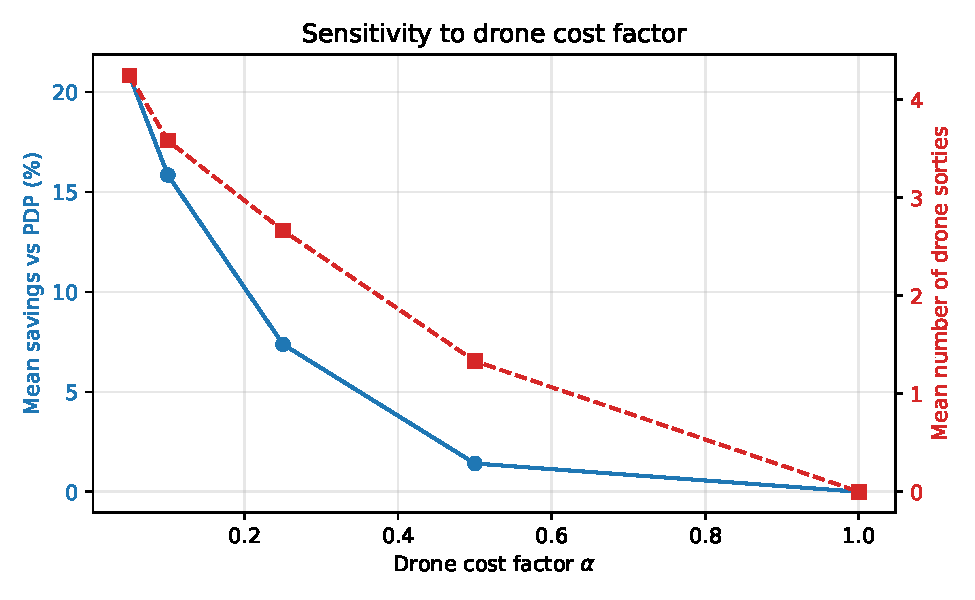
\includegraphics[width=0.6\textwidth]{figures/alpha.pdf}
\caption{Sensitivity of SPDP and number of sorties to the drone cost
factor $\alpha = c'/c$.}
\label{fig:sens_alpha}
\end{figure}

\section{Validation}
\label{sec:validation}

A reproduction of the paper's Table~A.5 is given in
Table~\ref{tab:validation}. We solve random seeds per $(n, \text{grid})$
pair for $n \in \{6, 8, 10\}$ and grid in $\{10, 20, 30\}$\,miles, the
sizes the paper itself reports. Number of seeds per cell is reduced at
larger $n$ to keep total runtime bounded ($5$ seeds at $n{=}6$, $3$ at
$n{=}8$, $2$ at $n{=}10$); the same Gurobi parameters are used throughout.

\begin{table}[h]
\centering
\caption{Mean SPDP and runtime per $(n, \text{grid})$ cell, from
\texttt{validation.py} ($5$ seeds at $n{=}6$, $3$ at $n{=}8$, $2$ at
$n{=}10$). Runtimes include model build; cells at $n{=}10$ reach the
$600$\,s solve limit (see text).}
\label{tab:validation}
\small
\begin{tabular}{@{}rrrrr@{}}
\toprule
$n$ & grid (mi) & mean SPDP (\%) & std (\%) & mean runtime (s) \\
\midrule
6  & 10 & $22.27$ & $6.94$ & $3.5$ \\
6  & 20 & $20.45$ & $5.68$ & $3.4$ \\
6  & 30 & $9.47$  & $5.31$ & $1.3$ \\
8  & 10 & $20.67$ & $8.41$ & $174.6$ \\
8  & 20 & $17.56$ & $10.42$ & $184.9$ \\
8  & 30 & $11.93$ & $1.59$ & $127.4$ \\
10 & 10 & $11.73$ & $9.39$ & $656.0$ \\
10 & 20 & $-5.09$ & $12.77$ & $959.7$ \\
10 & 30 & $16.15$ & $3.14$ & $591.0$ \\
\bottomrule
\end{tabular}
\end{table}

Across all nine cells the mean saving is $\approx 14\%$, with the largest
savings on the denser $10$\,mile grids where more eligible deliveries fall
within drone range. Two caveats apply at $n{=}10$. First, these solves reach
the $600$\,s time limit, so the reported objectives are best incumbents
rather than certified optima. Second, the $(n{=}10,\text{grid}{=}20)$ cell
shows a \emph{negative} mean SPDP ($-5.1\%$): because the \dapdp{} strictly
generalises the \pdp{} (the drone is optional), the true optimum can never
satisfy $z_{\dapdp}>z_{\pdp}$, so a negative saving is the signature of a
\dapdp{} solve that has not converged within the time limit and returned an
incumbent worse than its own \pdp{} baseline. This is exactly the
non-convergence case flagged in the assignment guidelines; it is resolved by
raising the time limit (or tightening the MIP gap) at $n{=}10$, not by any
change to the model, whose $z_{\dapdp}\le z_{\pdp}$ invariant is verified
directly in scenario~V6.

\section{Conclusions}

A faithful Python/Gurobi reproduction of the Mulumba--Diabat \dapdp{} MILP
is presented and verified. The seven verification scenarios all pass
their independent audits; SPDP increases with drone endurance and speed
and decreases with $\alpha$, in line with the paper's findings. Three
typographic ambiguities of the paper are documented and resolved.

The remaining gap relative to the paper is the absence of the ALNS
heuristic of their Section~4. The exact model is sufficient up to roughly
$n{=}10$--$12$ within seconds-to-minutes of solver time; the heuristic is
required only for the much larger test instances of their Section~5.

\begin{thebibliography}{1}
\bibitem{mulumba2024}
T.~Mulumba and A.~Diabat. \emph{Optimization of the drone-assisted pickup
and delivery problem}. Transportation Research Part E, 181:103377, 2024.
\end{thebibliography}

\end{document}
